\begin{filecontents*}{references.bib}
@article{nahmias1982perishable,
  author  = {Nahmias, Steven},
  title   = {Perishable Inventory Theory: A Review},
  journal = {Operations Research},
  volume  = {30},
  pages   = {680--708},
  year    = {1982}
}
@article{koenker1978regression,
  author  = {Koenker, Roger and Bassett, Jr., Gilbert},
  title   = {Regression Quantiles},
  journal = {Econometrica},
  volume  = {46},
  number  = {1},
  pages   = {33--50},
  year    = {1978}
}
@article{friedman2001gbm,
  author  = {Friedman, Jerome H.},
  title   = {Greedy Function Approximation: A Gradient Boosting Machine},
  journal = {The Annals of Statistics},
  volume  = {29},
  number  = {5},
  pages   = {1189--1232},
  year    = {2001}
}
@article{pedregosa2011sklearn,
  author  = {Pedregosa, Fabian and others},
  title   = {Scikit-learn: Machine Learning in {P}ython},
  journal = {Journal of Machine Learning Research},
  volume  = {12},
  pages   = {2825--2830},
  year    = {2011}
}
@article{holm1979simple,
  author  = {Holm, Sture},
  title   = {A Simple Sequentially Rejective Multiple Test Procedure},
  journal = {Scandinavian Journal of Statistics},
  volume  = {6},
  number  = {2},
  pages   = {65--70},
  year    = {1979}
}
@book{efron1993bootstrap,
  author    = {Efron, Bradley and Tibshirani, Robert J.},
  title     = {An Introduction to the Bootstrap},
  publisher = {Chapman \& Hall},
  address   = {New York},
  year      = {1993}
}
@article{makridakis2022m5,
  author  = {Makridakis, Spyros and Spiliotis, Evangelos and Assimakopoulos, Vassilios},
  title   = {{M5} Accuracy Competition: Results, Findings, and Conclusions},
  journal = {International Journal of Forecasting},
  volume  = {38},
  number  = {4},
  pages   = {1346--1364},
  year    = {2022}
}
@misc{favorita2018kaggle,
  author       = {{Corporaci{\'o}n Favorita}},
  title        = {Corporaci{\'o}n Favorita Grocery Sales Forecasting},
  howpublished = {Kaggle competition},
  year         = {2018},
  url          = {https://www.kaggle.com/c/favorita-grocery-sales-forecasting}
}
\end{filecontents*}

\documentclass[conference]{IEEEtran}
\IEEEoverridecommandlockouts

% --- Packages ---
\usepackage{cite}
\usepackage{amsmath,amssymb,amsfonts,amsthm}
\usepackage{graphicx}
\usepackage{textcomp}
\usepackage{xcolor}
\usepackage{booktabs}
\usepackage{multirow}
\usepackage{array}
\usepackage{tikz}
\usetikzlibrary{positioning,arrows.meta,fit,backgrounds,calc}
\usepackage{pgfplots}
\pgfplotsset{compat=1.18}
\usepgfplotslibrary{groupplots}

% One colour, marker and line style per event strength, used by every figure
\definecolor{cOne}{HTML}{56B4E9}
\definecolor{cTwo}{HTML}{009E73}
\definecolor{cThree}{HTML}{E69F00}
\definecolor{cFour}{HTML}{D55E00}
\definecolor{cA}{HTML}{4C566A}
\pgfplotsset{
  every axis/.append style={font=\footnotesize, tick label style={font=\scriptsize},
    label style={font=\footnotesize}, title style={font=\footnotesize\bfseries},
    grid style={gray!20}, major grid style={gray!20}},
  stOne/.style={color=cOne, mark=*, mark size=1.6pt, thick},
  stTwo/.style={color=cTwo, mark=triangle*, mark size=2pt, thick, dashdotted},
  stThree/.style={color=cThree, mark=diamond*, mark size=2pt, thick, densely dotted},
  stFour/.style={color=cFour, mark=square*, mark size=1.5pt, thick, densely dashed},
}
\usepackage{hyperref}
\hypersetup{hidelinks}

% Lets the author list break onto a second row (IEEEtran has no built-in command)
\makeatletter
\newcommand{\linebreakand}{%
  \end{@IEEEauthorhalign}
  \hfill\mbox{}\par
  \mbox{}\hfill\begin{@IEEEauthorhalign}}
\makeatother

\def\BibTeX{{\rm B\kern-.05em{\sc i\kern-.025em b}\kern-.08em
    T\kern-.1667em\lower.7ex\hbox{E}\kern-.125emX}}


\begin{document}

% ============================================================================
% TITLE & AUTHORS
% ============================================================================
\title{Event Signal Quality and Inventory Cost: A Simulation and Real-Data Study of Perishable Replenishment}

\author{
  \IEEEauthorblockN{Kritika Damahe}
  \IEEEauthorblockA{\textit{Department of Artificial Intelligence}\\
    \textit{and Data Science}\\
    Vishwakarma Institute of\\ Information Technology\\
    Pune, India\\
    kritika.22311693@viit.ac.in}
  \and
  \IEEEauthorblockN{Yash Kale}
  \IEEEauthorblockA{\textit{Department of Artificial Intelligence}\\
    \textit{and Data Science}\\
    Vishwakarma Institute of\\ Information Technology\\
    Pune, India\\
    yash.22311665@viit.ac.in}
  \and
  \IEEEauthorblockN{Abhijit Patil}
  \IEEEauthorblockA{\textit{Department of Artificial Intelligence}\\
    \textit{and Data Science}\\
    Vishwakarma Institute of\\ Information Technology\\
    Pune, India\\
    abhijit.22310820@viit.ac.in}
  \linebreakand
  \IEEEauthorblockN{Niharika Rahangdale}
  \IEEEauthorblockA{\textit{Department of Artificial Intelligence}\\
    \textit{and Data Science}\\
    Vishwakarma Institute of\\ Information Technology\\
    Pune, India\\
    niharika.22310975@viit.ac.in}
  \and
  \IEEEauthorblockN{Geetanjali Yadav}
  \IEEEauthorblockA{\textit{Department of Artificial Intelligence}\\
    \textit{and Data Science}\\
    Vishwakarma Institute of\\ Information Technology\\
    Pune, India\\
    geetanjali.yadav@viit.ac.in}
  \and
  \IEEEauthorblockN{Prema Kadam}
  \IEEEauthorblockA{\textit{Department of Artificial Intelligence}\\
    \textit{and Data Science}\\
    BRACT'S Vishwakarma Institute\\ of Technology\\
    Pune, India\\
    prema.kadam@vit.edu}
}

\maketitle

% ============================================================================
% ABSTRACT
% ============================================================================
\begin{abstract}
Demand forecasters for perishable goods are usually given event information (holidays, festivals, promotions) taken from a clean, after-the-fact calendar. At ordering time that information can be missing, late, false or mislabelled. We study when event signals reduce inventory cost and when imperfect signals do more harm than good. Three forecasters share one replenishment policy: one ignores events (A), one is trained on the true calendar (B), and one is trained on the signals as they would have been available at ordering time (C). In a simulation with strong events and clean signals, event-aware forecasting cuts cost by 36.9\% (cheaper in 20 of 20 seeds). With false-alarm-heavy signals, clean-calendar training costs 15.6\% more than ignoring events, and as-available training removes most of that harm (16.6\% cheaper than B). A sweep over event strength and false-alarm rate shows that all these effects scale with event strength: at the strength measured in real Favorita grocery data, every difference shrinks to 3.4\% or less. On Favorita, with 100 perishable series, event signals made no statistically distinguishable difference in cost once intervals are clustered by product. Event signals, and protection against their errors, are worth as much as events move demand.
\end{abstract}

\begin{IEEEkeywords}
perishable inventory, demand forecasting, event signals, signal quality, quantile forecasting, simulation.
\end{IEEEkeywords}

% ============================================================================
% I. INTRODUCTION
% ============================================================================
\section{Introduction}
\label{sec:intro}
Perishable retail has a narrow margin for error: over-ordering turns into waste and under-ordering turns into lost sales \cite{nahmias1982perishable}. Event information is a natural input to demand forecasts, but event features are usually built from a clean calendar that is known with certainty after the fact. In deployment the signal is different. Events are announced late, some are never announced, some announcements prove false, and labels can be wrong. A model that learned to trust a clean calendar may react strongly to a signal that is wrong.

This paper asks two questions.
\begin{enumerate}
    \item Does training on signals as they were actually available (arm C) reduce the cost harm of imperfect signals, compared with training on the clean calendar (arm B)?
    \item How does the answer depend on how strongly events move demand? When events barely matter, is any of this worth doing?
\end{enumerate}
Our contributions are as follows.
\begin{itemize}
    \item A controlled simulation of perishable replenishment (fixed shelf life, lead time, first-in-first-out stock) in which signal quality (misses, late announcements, false alarms, mislabelling) is a tunable input, and in which models are judged by inventory cost rather than forecast error alone (Section~\ref{sec:method}).
    \item A map of where event signals help, where they do nothing and where they hurt, over event strength and false-alarm rate (Section~\ref{sec:results}).
    \item A real-data check on Favorita grocery sales, where events are weak, with confidence intervals that account for demand being shared across seeds.
\end{itemize}
The claims concern operational cost under one heuristic replenishment policy, and we make no claim about deployed systems.

% ============================================================================
% II. RELATED WORK
% ============================================================================
\section{Related Work}
\label{sec:related}
Perishable inventory with fixed shelf life has a long theoretical tradition \cite{nahmias1982perishable}, in which ordering decisions depend on a demand forecast and on the ages of the units in stock. Modern replenishment pipelines commonly produce that forecast with machine-learned quantile models \cite{koenker1978regression, friedman2001gbm}, which map naturally onto newsvendor-style order-up-to levels. Calendar and event variables are standard inputs to such models, and public retail benchmarks such as Favorita \cite{favorita2018kaggle} and M5 \cite{makridakis2022m5} ship holiday and event calendars for that purpose.

We study a narrower question than event-aware forecasting in general. Given that event features are used, how does the quality of the signal at ordering time change the cost of the resulting orders, and does it matter whether the model saw the same kind of imperfect signal during training? We evaluate arms by simulated inventory cost, not only by forecast accuracy, and we vary event strength separately from signal quality so that the answer can be stated as a regime rather than a single number.

% ============================================================================
% III. METHODOLOGY
% ============================================================================
\section{Methodology}
\label{sec:method}

\subsection{Replenishment Problem}
One SKU is managed daily with lead time $L = 2$ days and shelf life $m = 4$ days. Stock is sold first-in-first-out, unmet demand is lost, and units reaching the end of their shelf life expire. Costs are 0.05 per unit-day held, 1.0 per lost unit and 0.6 per expired unit. Each day, after the delivery is received and before demand is served, an order $q$ is placed by an outdating-corrected order-up-to rule,
\begin{equation}
    q = \max\bigl(0,\; S - (\mathrm{IP} - \mathrm{E}_{L+1})\bigr),
\end{equation}
where $\mathrm{IP}$ is the inventory position, $\mathrm{E}_{L+1}$ is the projected FIFO expiry over the next $L+1$ days, and the order-up-to level $S$ is the $\tau$-quantile of the forecast of demand over days $t,\dots,t+L$. The rule is a heuristic and is not claimed to be optimal. All arms share it.

\subsection{Event Signals}
An announcement is a tuple $(\text{announce day}, \text{start}, \text{duration}, \text{type})$. On ordering day $t$ a forecaster sees only announcements with announce day $\le t$. The error process has four parts: missed events (probability $p_{\text{miss}}$), announcements delayed to the event's start day ($p_{\text{late}}$), spurious events at rate $\lambda$ per day, and spurious events labelled as the highest-uplift type ($p_{\text{mis}}$). Three signal conditions are used (Table~\ref{tab:conditions}); on-time announcements arrive 14 days ahead.

\begin{table}[t]
\centering
\caption{Signal conditions. Clean signals have no errors.}
\label{tab:conditions}
\setlength{\tabcolsep}{4pt}
\footnotesize
\begin{tabular}{@{}lrrrr@{}}
\toprule
\textbf{Condition} & $p_{\text{miss}}$ & $p_{\text{late}}$ & $\lambda$ (per day) & $p_{\text{mis}}$ \\
\midrule
clean       & 0   & 0   & 0    & 0   \\
imperfect   & 0.3 & 0.3 & 0.04 & 0.5 \\
false alarm & 0.1 & 0   & 0.08 & 0.8 \\
\bottomrule
\end{tabular}
\end{table}

\subsection{Forecasting Arms}
All arms use pooled gradient-boosted quantile regression (scikit-learn \texttt{HistGradientBoostingRegressor} with quantile loss \cite{pedregosa2011sklearn}), one model per quantile level, with the cumulative demand over days $t,\dots,t+L$ as target. Features use only demand before $t$, scaled by the trailing 28-day mean: SKU identifier, weekday, 7- and 28-day means, a seasonal-naive window and volatility. The event arms add, for each event type, the number of signalled days in the window.
\begin{itemize}
    \item \textbf{A (blind):} no event features.
    \item \textbf{B (clean-trained):} trained on the true calendar, every event announced 14 days ahead, then served the imperfect signal.
    \item \textbf{C (as-available-trained):} trained on the training-period part of the same signal realisation it is served with.
\end{itemize}
Under clean signals B and C see identical features and must give identical results, which serves as a built-in consistency check. The quantile $\tau$ is chosen separately for each arm and condition by validation-period simulated cost, and the test period is evaluated once.

\subsection{Demand Data}
\textbf{Synthetic.} Daily demand is negative-binomial with a mean equal to a SKU base level times a weekday profile, a linear trend and an event multiplier. Event uplifts vary by type and SKU, and 20\% of SKUs do not respond to events. Each seed is an independent world. \emph{Event strength} scales all event log-uplifts, with 1.0 the original simulation.

\textbf{Favorita.} Five Quito stores $\times$ 20 perishable items (100 series: 80 produce, 10 meats, 5 dairy, 5 poultry) over 742 days from 2015-08-01 to 2017-08-15, with 166 evaluated test days \cite{favorita2018kaggle}. Events come from the holiday calendar: national holidays (21 occurrences, 5 in the test period), national events (6 occurrences, 1 in test) and local holidays (2 occurrences, 0 in test). The April 2016 earthquake is excluded because it could not have been announced. Demand is fixed real sales, so seeds vary only the signal errors and the model fits. Recorded sales are censored by stockouts; zero-sale days are 0.4\% of the panel, which limits the bias.

\subsection{Statistics}
In the synthetic experiments each seed is an independent world, so the unit of analysis is the seed. The primary evidence is the per-seed 95\% $t$-interval of relative cost differences ($19$ degrees of freedom for $20$ seeds) and an exact two-sided sign-flip test. A comparison is called supported only when the interval excludes 0 and $p < 0.05$, and Holm's correction \cite{holm1979simple} is applied across the eight non-trivial comparisons at family-wise $\alpha = 0.05$. Bootstrap intervals over (seed, SKU) units \cite{efron1993bootstrap} are computed but are too narrow, since they ignore dependence, and are not used for conclusions.

On real data every seed shares the same demand, so seeds are not independent. There we resample products (20 clusters) or stores (5 clusters) instead, and treat the per-cluster $t$-interval as the conservative summary.

% ============================================================================
% IV. RESULTS
% ============================================================================
\section{Results and Discussion}
\label{sec:results}

\subsection{Synthetic: Strong Events, Three Conditions}
Table~\ref{tab:cost20} and Table~\ref{tab:stats20} report the 20-seed run with 40 SKUs and 161 evaluated test days.

\begin{table}[t]
\centering
\caption{Synthetic, 20 seeds: mean test cost summed over 40 SKUs.}
\label{tab:cost20}
\setlength{\tabcolsep}{5pt}
\footnotesize
\begin{tabular}{@{}lrrr@{}}
\toprule
\textbf{Condition} & \textbf{A (blind)} & \textbf{B (clean-trained)} & \textbf{C (as-available)} \\
\midrule
clean       & 17{,}748 & 11{,}208 & 11{,}208 \\
imperfect   & 17{,}748 & 17{,}992 & 17{,}134 \\
false alarm & 17{,}748 & 20{,}521 & 17{,}121 \\
\bottomrule
\end{tabular}
\end{table}

\begin{table*}[t]
\centering
\caption{Synthetic, 20 seeds: paired relative test-cost differences (negative = first arm cheaper). Interval: per-seed 95\% $t$-interval. $p$: exact sign-flip test. Holm: adjusted over the eight comparisons shown. Clean C vs B is omitted because the two arms are identical by design; clean B vs A therefore equals clean C vs A and is kept as a separate hypothesis, which makes the correction slightly conservative.}
\label{tab:stats20}
\setlength{\tabcolsep}{5pt}
\footnotesize
\begin{tabular}{@{}llrrrrrl@{}}
\toprule
\textbf{Condition} & \textbf{Comparison} & \textbf{Estimate} & \textbf{Interval} & \textbf{$p$} & \textbf{First cheaper} & \textbf{Holm $p$} & \textbf{Supported?} \\
\midrule
clean       & C vs A & $-36.9\%$ & $[-38.68, -33.75]$ & $1.9\times10^{-6}$ & 20/20 & $1.5\times10^{-5}$ & Yes \\
clean       & B vs A & $-36.9\%$ & $[-38.68, -33.75]$ & $1.9\times10^{-6}$ & 20/20 & $1.5\times10^{-5}$ & Yes \\
false alarm & C vs B & $-16.6\%$ & $[-19.63, -12.64]$ & $1.9\times10^{-6}$ & 20/20 & $1.5\times10^{-5}$ & Yes \\
false alarm & B vs A & $+15.6\%$ & $[+8.21, +25.60]$ & $1.5\times10^{-4}$ & 2/20  & $7.6\times10^{-4}$ & Yes (B worse) \\
imperfect   & C vs B & $-4.8\%$  & $[-8.09, -0.08]$  & 0.047 & 15/20 & 0.188 & Marginal, fails Holm \\
imperfect   & C vs A & $-3.5\%$  & $[-7.73, +0.27]$  & 0.063 & 15/20 & 0.189 & No \\
false alarm & C vs A & $-3.5\%$  & $[-8.25, +2.55]$  & 0.287 & 15/20 & 0.574 & No \\
imperfect   & B vs A & $+1.4\%$  & $[-4.38, +6.29]$  & 0.716 & 11/20 & 0.716 & No \\
\bottomrule
\end{tabular}
\end{table*}

Four findings follow. First, accurate signals pay off strongly: clean C versus A is $-36.9\%$. Second, clean-calendar training with false-alarm-heavy signals is worse than ignoring events ($+15.6\%$), and as-available training removes most of that harm ($-16.6\%$ versus B). Third, with mixed, moderate errors the advantage of C over B is small and does not survive multiplicity correction. Fourth, neither imperfect condition shows that using imperfect signals beats ignoring them: C versus A is not supported in either.

\subsection{Synthetic: Event Strength $\times$ False-Alarm Rate}
Event strength scales the generator's event log-uplifts, and 0.1 is roughly the level measured in the Favorita panel. The false-alarm rate is $\lambda$, with $p_{\text{miss}} = 0.1$ and $p_{\text{mis}} = 0.8$ throughout, so the $\lambda = 0$ cells still contain 10\% missed events and are not the clean condition of Table~\ref{tab:conditions}. Each cell is the mean per-seed relative cost difference over 10 seeds (Table~\ref{tab:grid}, Fig.~\ref{fig:grid}). Sign-flip $p$-values are not corrected for multiplicity; with 10 seeds the smallest attainable value is 0.002, reached whenever all ten seeds agree.

\begin{table*}[t]
\centering
\caption{Event strength $\times$ false-alarm rate $\lambda$ (synthetic, 10 seeds): mean per-seed relative test-cost difference in \%. Negative means the first arm is cheaper.}
\label{tab:grid}
\setlength{\tabcolsep}{4pt}
\footnotesize
\begin{tabular}{@{}l rrrr @{\hspace{12pt}} rrrr @{\hspace{12pt}} rrrr@{}}
\toprule
 & \multicolumn{4}{c}{\textbf{C vs A}} & \multicolumn{4}{c}{\textbf{B vs A}} & \multicolumn{4}{c}{\textbf{C vs B}} \\
\cmidrule(lr){2-5}\cmidrule(lr){6-9}\cmidrule(l){10-13}
\textbf{Strength} & 0 & .04 & .08 & .16 & 0 & .04 & .08 & .16 & 0 & .04 & .08 & .16 \\
\midrule
0.1  & $-3.0$  & $-2.2$  & $-1.5$ & $-1.4$ & $-3.4$  & $-2.3$ & $-1.0$ & $+0.1$  & $+0.4$ & $+0.1$ & $-0.5$  & $-1.5$  \\
0.25 & $-5.8$  & $-3.9$  & $-2.9$ & $-2.5$ & $-6.1$  & $-3.6$ & $-0.5$ & $+3.3$  & $+0.3$ & $-0.3$ & $-2.4$  & $-5.6$  \\
0.5  & $-14.2$ & $-9.3$  & $-2.8$ & $-3.2$ & $-14.9$ & $-6.5$ & $+5.7$ & $+12.5$ & $+0.9$ & $-3.0$ & $-7.9$  & $-13.7$ \\
1.0  & $-32.4$ & $-15.5$ & $+0.0$ & $-1.6$ & $-34.5$ & $-9.2$ & $+20.0$ & $+40.0$ & $+3.2$ & $-7.0$ & $-16.1$ & $-29.4$ \\
\bottomrule
\end{tabular}
\end{table*}

\begin{figure*}[t]
\centering
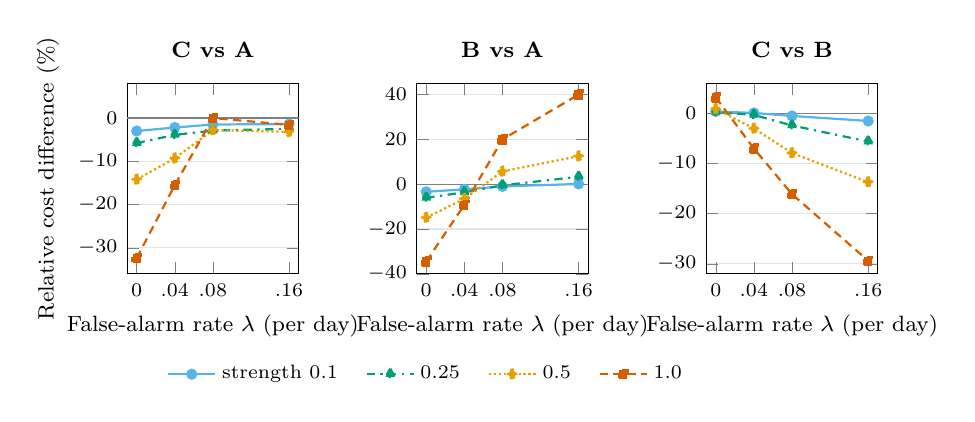
\begin{tikzpicture}
\begin{groupplot}[group style={group size=3 by 1, horizontal sep=1.5cm},
  width=0.31\textwidth, height=4.0cm, xmin=-0.01, xmax=0.17, xtick={0,0.04,0.08,0.16},
  xticklabels={0,.04,.08,.16}, ymajorgrids, xlabel={False-alarm rate $\lambda$ (per day)}]
\nextgroupplot[title={C vs A}, ylabel={Relative cost difference (\%)}, ymin=-36, ymax=8,
  legend style={at={(1.75,-0.42)}, anchor=north, legend columns=4, draw=none, font=\scriptsize, /tikz/every even column/.append style={column sep=8pt}}]
\addplot[gray, thin, forget plot] coordinates {(-0.01,0) (0.17,0)};
\addplot[stOne] coordinates {(0,-3.0) (0.04,-2.2) (0.08,-1.5) (0.16,-1.4)}; \addlegendentry{strength 0.1}
\addplot[stTwo] coordinates {(0,-5.8) (0.04,-3.9) (0.08,-2.9) (0.16,-2.5)}; \addlegendentry{0.25}
\addplot[stThree] coordinates {(0,-14.2) (0.04,-9.3) (0.08,-2.8) (0.16,-3.2)}; \addlegendentry{0.5}
\addplot[stFour] coordinates {(0,-32.4) (0.04,-15.5) (0.08,0.0) (0.16,-1.6)}; \addlegendentry{1.0}
\nextgroupplot[title={B vs A}, ymin=-40, ymax=45]
\addplot[gray, thin] coordinates {(-0.01,0) (0.17,0)};
\addplot[stOne] coordinates {(0,-3.4) (0.04,-2.3) (0.08,-1.0) (0.16,0.1)};
\addplot[stTwo] coordinates {(0,-6.1) (0.04,-3.6) (0.08,-0.5) (0.16,3.3)};
\addplot[stThree] coordinates {(0,-14.9) (0.04,-6.5) (0.08,5.7) (0.16,12.5)};
\addplot[stFour] coordinates {(0,-34.5) (0.04,-9.2) (0.08,20.0) (0.16,40.0)};
\nextgroupplot[title={C vs B}, ymin=-32, ymax=6]
\addplot[gray, thin] coordinates {(-0.01,0) (0.17,0)};
\addplot[stOne] coordinates {(0,0.4) (0.04,0.1) (0.08,-0.5) (0.16,-1.5)};
\addplot[stTwo] coordinates {(0,0.3) (0.04,-0.3) (0.08,-2.4) (0.16,-5.6)};
\addplot[stThree] coordinates {(0,0.9) (0.04,-3.0) (0.08,-7.9) (0.16,-13.7)};
\addplot[stFour] coordinates {(0,3.2) (0.04,-7.0) (0.08,-16.1) (0.16,-29.4)};
\end{groupplot}
\end{tikzpicture}
\caption{Mean relative test-cost difference (negative = first arm cheaper) against false-alarm rate, one line per event strength (synthetic, 10 seeds). Strength 0.1 is roughly the level measured in Favorita.}
\label{fig:grid}
\end{figure*}

The map has four features. The benefit of events grows with strength, from about 3\% to about 32\% at zero false alarms. The harm from false alarms also grows with strength: at strength 1.0 and $\lambda = 0.16$, clean-trained B costs 40\% more than ignoring events. The protection from as-available training (C versus B) grows with both strength and false-alarm rate, and is near zero or slightly adverse ($+0.3\%$ to $+3.2\%$) when there are no false alarms. At strength 0.1 every difference is within 3.4\%, which is the regime Favorita falls into.

\subsection{Real Data: Favorita}
Table~\ref{tab:favcost} and Table~\ref{tab:favci} give the 20-seed Favorita run on 100 series.

\begin{table}[t]
\centering
\caption{Favorita, 20 seeds: mean test cost summed over 100 series.}
\label{tab:favcost}
\setlength{\tabcolsep}{5pt}
\footnotesize
\begin{tabular}{@{}lrrr@{}}
\toprule
\textbf{Condition} & \textbf{A (blind)} & \textbf{B (clean-trained)} & \textbf{C (as-available)} \\
\midrule
clean       & 127{,}203 & 127{,}909 & 127{,}909 \\
imperfect   & 127{,}203 & 128{,}359 & 127{,}467 \\
false alarm & 127{,}203 & 128{,}203 & 128{,}042 \\
\bottomrule
\end{tabular}
\end{table}

\begin{table}[t]
\centering
\caption{Favorita: relative cost difference (negative = first arm cheaper) with 95\% intervals clustered by item (20 clusters).}
\label{tab:favci}
\setlength{\tabcolsep}{3pt}
\footnotesize
\begin{tabular}{@{}llrrr@{}}
\toprule
\textbf{Condition} & \textbf{Comparison} & \textbf{Est.} & \textbf{Cluster bootstrap} & \textbf{Per-cluster $t$} \\
\midrule
clean       & B/C vs A & $+0.6\%$ & $[-0.4, +1.7]$ & $[-0.5, +1.0]$ \\
false alarm & C vs A   & $+0.7\%$ & $[-0.2, +1.6]$ & $[-0.1, +1.2]$ \\
false alarm & B vs A   & $+0.8\%$ & $[-0.2, +1.9]$ & $[-0.2, +1.2]$ \\
imperfect   & C vs A   & $+0.2\%$ & $[-0.3, +0.7]$ & $[-0.2, +0.6]$ \\
imperfect   & B vs A   & $+0.9\%$ & $[-0.0, +2.0]$ & $[-0.5, +1.3]$ \\
imperfect   & C vs B   & $-0.7\%$ & $[-1.4, -0.0]$ & $[-0.9, +0.1]$ \\
\bottomrule
\end{tabular}
\end{table}

Event signals did not measurably change cost on Favorita: every item-clustered $t$-interval for events versus ignoring them includes zero, and the point estimates are slightly positive, meaning events are slightly worse. The ordering seen in simulation appears in miniature, since under imperfect signals C is slightly cheaper than B ($-0.7\%$), but the evidence is weak. The per-item $t$-interval includes zero, and with store clustering (5 clusters) the interval is $[-1.4, +0.2]$ for C versus B. With store clustering the cluster bootstrap for imperfect B versus A is $[+0.2, +1.3]$, but its per-store $t$-interval $[-0.5, +2.0]$ includes zero.

The weak effect has plausible reasons. National holidays raise sales by only about 9\% (training-period mean log-uplift $+0.087$), national events by about 0\% ($-0.008$), the test period holds only six events, and 80\% of the series are produce, whose demand is steady across the calendar. With so little signal to learn from, the extra event features add more noise than information. With clean signals, cost on event-window days fell by 0.75\% against A, but cost on the remaining days, which carry 77\% of the cost, rose by 0.95\%, giving the slightly positive estimates for B and C against A. Finally, widening the quantile grid to include 0.95 and 0.975 did not change the picture: every arm still selects $\tau = 0.90$, so the earlier grid was not the constraint.

\subsection{Discussion}
\textbf{Answers to the two questions.} Training on as-available signals reduces the cost of imperfect signals, and the benefit grows with the false-alarm rate. It is strongly supported in simulation when false alarms are common, weak when errors are mixed and moderate, and not distinguishable from zero on Favorita. The size of every effect is governed by event strength: when events move demand a lot, accurate signals are worth tens of percent and false alarms can cost as much, whereas when events move demand by under about 10\%, the whole question is worth a few percent at most.

\textbf{Practical reading.} Before investing in event features or in the quality of an event feed, estimate how much events move demand for the product in question. If the uplift is small, a blind forecaster is as good. If it is large, clean signals are valuable, and training the forecaster on realistic signals is a cheap way to avoid doing worse than a blind forecaster when signals are unreliable.

\textbf{Scope.} The Favorita result concerns everyday perishables, mostly produce, around national and local holidays. It should not be read as ``events never help in real retail.''

\subsection{Limitations}
\begin{enumerate}
    \item \textbf{Design favours C in part.} C is trained and evaluated on the same error process, and its advantage when that process shifts between training and deployment has not been tested.
    \item \textbf{One policy and one cost structure.} All arms share one heuristic order-up-to rule, with lead time 2, shelf life 4 and fixed cost ratios. Other policies or cost ratios could change the sizes of the differences.
    \item \textbf{Simplified operations.} A single SKU at a single echelon, with no capacity limits, ordering costs, substitution or supplier variability.
    \item \textbf{Censored demand.} Real sales understate demand during stockouts (0.4\% of Favorita series-days are suspected stockouts).
    \item \textbf{Few clusters.} Twenty seeds is a modest number, and store-level clustering on Favorita has only five clusters, for which the smallest attainable sign-flip $p$ is 0.0625.
    \item \textbf{Panel composition.} Eighty of the 100 Favorita series are produce, from a single city.
    \item \textbf{Grid size.} The strength $\times$ false-alarm grid uses 10 seeds, and its $p$-values are uncorrected.
    \item \textbf{One real data set, with weak events.} Favorita's events are weak, so it cannot show whether the simulated benefit of accurate signals holds on real data when events are strong. Scheduled, strong events, such as the SNAP benefit days in M5 \cite{makridakis2022m5}, are a natural next test.
    \item \textbf{Library-version sensitivity.} Results are deterministic in a fixed environment, but the gradient-boosting fits change with the scikit-learn version: an earlier 5-seed run under scikit-learn 1.9.1 gives per-seed costs up to 10\% different from the same seeds under 1.8.0. All reported results use one pinned environment, recorded with each run.
    \item \textbf{No pre-registration.} The hypotheses were set during prototype design.
\end{enumerate}

% ============================================================================
% V. CONCLUSION
% ============================================================================
\section{Conclusion}
\label{sec:conclusion}
Event signals are worth about as much as events move demand, and imperfect signals can destroy that value. In simulation, accurate event information cut inventory cost by 37\%, and false-alarm-heavy signals made a clean-trained model 16\% worse than ignoring events, while a model trained on realistic signals recovered most of that loss. On real Favorita perishables, where events move demand by less than 10\%, none of it mattered. A map over event strength and false-alarm rate tells practitioners which regime they are in. The next step is a real-data case with strong, scheduled events, to check whether the simulated map predicts the cost differences observed there. Code, configurations and saved results are available at \url{https://github.com/kritikadamahe/Nexora/tree/main/research/event_signal_inventory}.

% ============================================================================
% REFERENCES
% ============================================================================
\bibliographystyle{IEEEtran}
\bibliography{references}

\end{document}
